\documentclass[a4paper,12pt,twoside,leqno]{article}
\usepackage[marginratio={5:5, 5:5}, textwidth=150mm, ]{geometry}


\pagenumbering{gobble}
\usepackage{amssymb}
\usepackage{xcolor}
\usepackage{amsmath}
\usepackage{epigraph} 
\usepackage{mhchem}

\usepackage{tikz}
\usetikzlibrary{quotes}
\usetikzlibrary{automata, arrows.meta, positioning}
\bibliographystyle{apalike}
\usepackage[authoryear]{natbib}
\usepackage[colorlinks=true, linkcolor=blue, citecolor=blue, urlcolor=blue]{hyperref}


\title{\textbf{Short remarks on organizational closure}}
\author{Gonçalo Braga}

\begin{document}
\maketitle


\begin{abstract}Some notes on the concept of organizational closure (as in closure of constraints, closure to efficient causation, and similar ones), touching upon some other potentially related things along the way, which I might find important to mention. Hopefully, in not too rant-ish a manner. Majority of examples and discussion is done around minimal organisms or systems which could be argued to exemplify similar properties (e.g. unicellular, proto-cells, autocatalytic biomolecular condensates - think for instance about similar systems to coacervates - but under which some of the catalysts would also serve as scaffold and client molecules). Mostly to be developed over time, in hopes of sorting out some confusion I might have.
\end{abstract}


\paragraph*{}


\section{Biological organization as self-constraint}

\epigraph{An organized being is then not a mere machine, for that has merely a motive power; but it possesses in itself formative power, and such a one, moreover, as it communicates to the materials, which do not possess it (it organizes them). Thus it requires no other purposive principle for its maintenance than the one which it itself produces. In such a product of nature, every part is thought as if it exists only by means of all the others, and so exists for the sake of the others and the whole, i.e., as an instrument (organ). And this reciprocal causation of the parts in the whole distinguishes a machine from an organized being. In the former, the parts only act on one another in turn (so that one part is the instrument of the motion of the other); but in the latter, the parts are reciprocally cause and effect of their form.}{\cite{Kant1790-KANCOJ-2}}


Organisms are said to be systems which can both construct and maintain themselves. They aren’t merely self-organizing, as they can also maintain the capacity to self-organize. And for such to happen, they must have some type of closure at the organizational level. They must maintain this capacity from within their organization (see for instance \cite{rosen1991life, maturana2012autopoiesis, varela2025principles, moreno2015biological, kauffman2000investigations, deacon2021molecules}). It is in this sense, that organisms are said to be self-determined, self-constrained, to be both the means and the end. The constraints in an organism are said to be mutually dependent. They hold a dialectical relation with respect to each other, and as such can’t exist independently. Through this view, we get to notions such as closure of constraints, where each constraint in the organism’s organization needs to produce at least another one (e.g. \cite{montevil2015biological, moreno2015biological, mossio2013emergence}). This is how organisms achieve some type of causal closure, and how a minimal form of autonomy is achieved \citep{moreno2015biological}. It should be noted that this isn’t about physical closure, nor is it about a system becoming isolated from its environment. Much to the contrary, any system which is to achieve organizational closure must necessarily be at far-from-equilibrium conditions. It must continually do work in a constrained manner in order for closure to be maintained, and being thermodynamically open is a necessity. Furthermore, one shouldn’t associate closure to permanence, neither of constraints nor of relations between these. What needs to be achieved is continuity of this organization (maintenance of organizational closure), regardless of what constraints might be present. In this sense, organizational closure is probably the only property which can be said to be invariant over time in an organism.

\paragraph*{}

\citet{Kant1790-KANCOJ-2} was perhaps one of the first to capture this notion generally, along with the notion of \textit{self-organization} which now might merely stand for systems which come to be more organized, but which can’t maintain the constraints that allow such organization (these eventually dissipate away).
It's through this organization, which is inherently circular and impredicative, that the concept of intrinsic teleology emerges (e.g. \citet{mossio2017makes, weber2002life, di2005autopoiesis, garcia2024origins, garcia2022naturalisation, jonas2001phenomenon}), as Kant was preoccupied with \citep{Kant1790-KANCOJ-2, weber2002life}.

\section{Circularity of what exactly?}

One doesn't need to go beyond unicellularity to appreciate how complex organisms are. Consider the following passage written in \cite{tartar1961biology} about the large cilitate (albeit unicellular - on the order of 1 mm) \emph{Stentor coeruleus
}:

\begin{quote}
When a sample of \emph{coeruleus} is set aside for a week or two without
added nutrients the animals starve until individuals are produced
which are much smaller than normal daughter cells. Starting with
these starvation dwarfs, I cut off substantial portions of the posterior
pole and found that pieces as small as $75\,\mu m$ in diameter or only
$1/123$rd the volume of large, pre-starvation stentors, could regenerate completely and survive for over 6 days.
\end{quote}

This is a single-celled organism which exemplifies remarkable regeneration capabilities (see for instance \cite{slabodnick2014stentor, tartar1961biology, marshall2021regeneration}).

Asking how it can regenerate in such manner, is not a very different question from asking how it can maintain organizational closure. It is equivalent to asking how can said systems keep on producing every constraint from within themselves even when perturbed drastically.

I have now mentioned a couple of times that causal closure happens at the constraint level. What does this really mean? At a first glance, one might perhaps state that organisms are composed by networks of processes which produce every component in said network, such that the network can maintain itself. Notwithstanding the generality present here, we can ask: "Every component?". That can't be correct. Being thermodynamically open, it's clear that not every component is produced from within the system. This is where the notion and concept of a constraint is helpful. Constraints can be generally seen as physical objects or structures, which impose some limits on how an underlying process at the detailed dynamical level can change. Regarding a formalist description (and particularly if one takes a dynamical systems theory approach), said constraints appear as externally given, under boundary conditions, control parameters, etc; and these can change but not on the same temporal scale as the objects which are being described under the corresponding dynamical laws at the detailed dynamics level\footnote{One can of course also assume some reflexivity conditions, such that the states transversed will also act as transformations on the underlying dynamics (i.e. for instance states will lead to a change of the form of a corresponding set of coupled ODEs, to a change of control parameters, etc).}. In the circunstances where the corresponding constraints limit the underlying dynamics so as to leverage them into producing a set of constraints which can keep on doing the same thing (i.e. channeling work into producing further constraints), we say that the system has closure of constraints\footnote{Of course there's always the problem of understanding what to consider as a constraint (and as the constrained), through which observables to have such description, all of which are always dependent on the modeller's intentions to capture the behaviour of a certain phenomenon. Additionally, causality is a contentious issue (e.g. \cite{mossio2013emergence, craver2007top}).} (e.g. \cite{montevil2015biological, moreno2015biological, mossio2013emergence}; not exhaustive at all - majority of other references to be found therein).

Afterall, there's an infinitude of dynamical systems in Nature which are self-organizing to a certain degree \citep{glansdorff1973thermodynamic}, but in these the constraints which allow for such self-organization eventually dissipate away. Organisms, to this extent, can be said to be systems composed by coupled self-organizing processes which compensate for each other’s dissipative tendencies. Not only do they maintain this capability for self-organization, but they get better and more complex at it.

Someone's work which captures this notion of organizational closure in an interesting albeit very abstract manner, is that of \citet{rosen1991life}'s. \citet{rosen1991life} makes heavy use of Aristotelian (be)causes, using efficient and material causes to capture the notion of constraints and that of the constrained, respectively\footnote{\citet{rosen1991life} uses these explicitly, whilst formal and final causes are either used implicitly or not at all. Additionally, check \cite{hofmeyr2017basic, hofmeyr2018causation, hofmeyr2021biochemically} for a general contextualization of these abstract relational models w.r.t. cell biochemistry, with the use of formal cause. Furthermore, \cite{hofmeyr2021biochemically} represents a few more diagrams which are closed to efficient causation. On the issue of formal causation, \cite{hofmeyr2018causation, hofmeyr2021biochemically} makes the distinction between intrinsic and extrinsic formal cause, which I presume is based on \cite{oderberg2021formal}. \cite{oderberg2021formal} also seems to sub-divide accidental (intrinsic) into contigent and necessary. On top of me not having a proper philosophical background to fully understand what \cite{oderberg2021formal} is conveying, majority of examples are every-day ones, to the extent that it's very hard to map these concepts into their suitable form to be used in a molecular context. As it stands, these don't seem to provide enough conceptual value. The same applies to the distinction between closure and openness to formal cause, which seems to only be given a few paragraphs over \cite{hofmeyr2021biochemically}. To this same extent, I found \cite{bich2016biological} to provide potentially the same distinction between closure and openness to formal cause without use of Aristotelian causes (i.e. with closure and openness to formal cause, seeming to be equivalent respectively to, a system which only has a constitutive regime, and one which on top of a constitutive regime has some regulatory constraints).}. The central thesis that \citet{rosen1991life} puts forward, is that every material system which is closed to efficient causation is an organism. Represented in the next diagram, is the (M, R)-system which \citet{rosen1991life} chose to represent such causal regime:

\begin{figure}[h]
\begin{center}
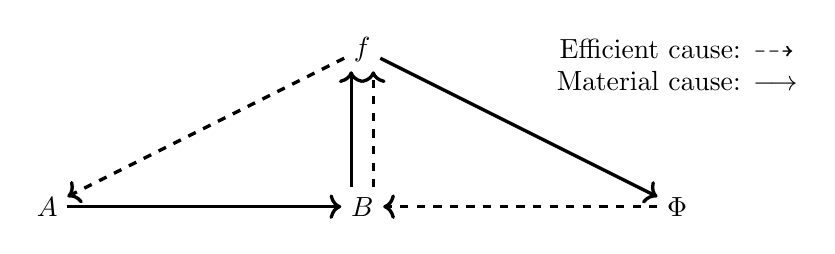
\begin{tikzpicture}[scale = 2]
	\node (eff) at (4, 1) {Efficient cause: $\dashrightarrow$};
	\node (matt) at (4, 0.8) {Material cause: $\longrightarrow$};
    \node (A) at (0,0) {$A$};
    \node (B) at (2,0) {$B$};
    \node (Phi) at (4, 0) {$\Phi$};
    \node (f) at (2, 1) {$f$};
    \draw[->, very thick] (A) -- (B);
    \draw[->, very thick] (f) -- (Phi);
    \draw[dashed, ->, very thick] (f) -- (A);
    \draw[dashed, ->, very thick] (Phi) -- (B);
    \draw[->, very thick] ([xshift=-2pt]B.north) -- ([xshift=-2pt]f.south);
    \draw[dashed, ->, very thick] ([xshift=2pt]B.north) -- ([xshift=2pt]f.south);  
\end{tikzpicture}
\end{center}
\end{figure}

where the mappings $f: A \rightarrow B$ ("metabolic" mapping, usually interpreted as a set of catalysts $f$ (efficient cause) acting upon a set of substrates $A$ (material cause) transforming these into products $B$), with $f \in H(A, B)$, $\Phi: B \rightarrow H(A, B)$ ("repair" mapping; supposed to reflect the replenishment or regeneration of $f$), such that $\Phi(b) = f$,  and $B: f \rightarrow \Phi$ (the "replication" mapping $\beta: H(A, B) \rightarrow H(B, H(A, B))$ such that $\beta(f) = \Phi$) being a very restricted mapping as $\Phi(b) = f$ is only to have one solution, are producing each other in a manner such that the system is closed to efficient causation. Interpretations of this (M, R)-system are readily available in the literature, for instance in \cite{letelier2006organizational, soto2011ouroboros, cardenas2010closure}, along with better contextualization of other (M, R)-systems (and other systems closed to efficient causation) in \cite{hofmeyr2021biochemically}.\paragraph*{}
I don't intend to prolong myself too much here, but let me make a few remarks. First, to me it's unclear what these relational abstract diagrams are actually supposed to capture beyond what's trivially visible. Distinctions between different types of entailment are very discernible. For instance, one can make diagrams under which systems which have some type of circular organization are very easy to distinguish. This is the case when comparing a system where a set of substrates are transformed into products which then serve as substrates again under a different catalyst, for which this type of relation repeats to the extent that the system is closed to material causation (but under which no further catalysts are being produced); and another one which is closed to efficient causation (think for example about an autocatalytic set, where the catalysts (or the efficient causes) produce each other collectively from a given set of substrates; albeit here one should also provide proper co-localization constraints, such that there are some type of constraints on diffusion of the corresponding catalysts and metabolites - e.g. some by-product of the autocatalytic network self-assembling into a membrane or capsid-like structure; some type of phase separation event by supersaturation conditions, as happens in LLPS, leading to some type of constraint on diffusion, etc).\\
Moreover, these diagrams themselves (and the usual interpretations accompanying them) are supposed to be very general I assume. See for instance \cite{hofmeyr2021biochemically} for a contextualization of these with the respect to cell biochemistry. They aren't supposed to give a similar view to the one we get when describing reaction networks, for instance, or any dynamical approach for that manner. They are apparently supposed to capture very general functional relationships between components, processes, constraints, etc. What this might mean more concretely, is what I'm not sure about. In my view, it only stands as a way to exemplify organizational closure in a very general manner. That's the only conceptual work it seems to have associated to it.\\
What's the role that organizational closure should have? Merely a principle which should be kept in the back of our minds when modelling some biological system (i.e. any sub-system or set of mechanisms (mechanism as in \cite{bich2021mechanism, bechtel2011mechanism} - mechanism need not be reductive) which are modelled at any time, should be contextualized with them being a sub-part of an autonomous system, that has its mechanisms organized in such a manner to maintain said autonomy)? It's not by mistake that \cite{rosen1991life} conjectures that organisms (and complex systems by that manner - here regarding Rosennean complexity which is different from more traditional notions \citep{rosen1991life}) have no largest model. We have a practically infinite (perhaps the best term here would actually be \textit{indefinite}) amount of ways of decomposing such systems, with corresponding observables which are to be tracked, without ever capturing the full behaviour of such systems. Most of these models can then only be taken as tools, with an appropriate range of applicability, and potentially complementing each other.\\
And yet, what does one make out of organizational closure? From the organizational account, one gets the notion that this is indeed the defining property of organisms, as in the general case of what an organism is. In fact, it seems to be the only property which is invariant over time in organisms, nevermind the practical difficulties in how to appropriately describe what's to be considered as a constraint (and as corresponding processes being constrained) in any given scenario. The question then is: is organizational closure capturable? If not, why so?\\
Without taking it into account, it feels as if one is generally studying processes as if they aren't happening in an organism. It is to this extent, that I feel that organizational closure puts "systems" into "systems biology".

\section{What should organizational closure provide?}


\addcontentsline{toc}{section}{References}
\bibliography{closure_refs}


\end{document}
